\documentclass[twocolumn,11pt]{article}
\usepackage[top=0.55in,bottom=0.55in,left=0.75in,right=0.75in]{geometry}
\usepackage{amsmath}
\usepackage{amsfonts}
\usepackage{amssymb}
\usepackage{amsthm}
\usepackage{amsrefs}
\usepackage{amscd}
\usepackage{microtype}
\usepackage{url}
\usepackage{graphicx}
\setlength{\emergencystretch}{3em}
\newcommand{\colfigwidth}{0.98\linewidth}

\title{AIM5070\_41: Spoken Language Processing - HW1}
\author{Morton Jacob Richard \and Student ID: 2026712407 \and Email: jacobmorton@skku.edu}
\date{March 22, 2026}

\begin{document}
\maketitle

\section{Introduction}

\emph{Lightweight keyword spotting} (KWS) on Google Speech Commands v2 (GSC~v2) classifies $1$~s, $16$~kHz clips into twelve labels: ten commands (\texttt{yes}, \texttt{no}, \texttt{up}, \texttt{down}, \texttt{left}, \texttt{right}, \texttt{on}, \texttt{off}, \texttt{stop}, \texttt{go}), plus \texttt{silence} and \texttt{unknown} (remaining vocabulary collapsed). This fixed-vocabulary task for on-device KWS (cf.\ Google, \emph{Streaming Keyword Spotting on Mobile Devices}). Inputs are \emph{log mel} spectrograms ($40$~ms window, $20$~ms hop, $80$ bins). We train under a $\leq 2.5$M parameter budget with one augmentation, two regularizers, TensorBoard logging, and a held-out test evaluation.

\section{Method}

\paragraph{Setup.}
I used an encoder--classifier with cross-entropy on 12 logits ($\sim$1.33M parameters). This was my first PyTorch Lightning project. Small amount (\textless 25\%) of the code was AI-assisted, mainly Lightning. Architecture and audio choices are my own. GSC data loading with AudioLoader~\cite{audioloader}. Training and evaluation code reimplemented from the nnAudio KWS Lightning tutorial~\cite{nnaudio_tutorial}. Metrics: TensorBoard. Training time: $\sim$3~h on Apple M5 (10 cores, 32~GB).

\paragraph{Model.}
\emph{Encoder:} Log-mel $\approx 50$~frames/s, $80$ mels $\rightarrow$ 1D conv embedding $\rightarrow$ dilated ConvNeXt-style blocks. The multi-dilation blocks are inspired by Multi-receptive-field fusion in Hi-FiGAN and the ConvNeXt-style stacks are inspired by VOCOS. Conv1D downsampling ($7$ kernel size, $2$ stride) plus further ConvNeXt stacks reduce rate to $12.5$~frames/s before pooling, to limit information loss versus pooling from full rate. Low frame rate also reduces computaion cost for the Bidirectional GRU on the last stage. \emph{Head:} pool frame embeddings, then an MLP $\rightarrow$ 12 logits. Cross-entropy loss is used on the softmax probabilities on the output of the MLP. \emph{Augmentation:} waveform TimeMask (SpecAugment-style). \emph{Regularization:} head dropout (0.2), AdamW weight decay, cosine LR schedule.

\section{Results}

\begin{table}[t]
    \centering
    \caption{Dataset split accuracy and model size.}
    \label{tab:acc}
    \begin{tabular}{lr}
      \hline
      Metric & Value \\
      \hline
      Train accuracy    & $0.9974$ \\
      Validation accuracy & $0.9744$ \\
      Test accuracy     & $0.9697$ \\
      Num.\ parameters  & $1.33$M \\
      \hline
    \end{tabular}
  \end{table}

Table~\ref{tab:acc} summarizes epoch-level training accuracy (final epoch), best-tracked validation accuracy during training, and held-out test accuracy from checkpoint evaluation, along with the total parameter count. I was able to achieve the required test accuracy of $0.9697$ with a small model and a single data augmentation, along with a small amount of regularization.


Figures~\ref{fig:train}--\ref{fig:test_no} show TensorBoard traces, TimeMask, the test confusion matrix, and test examples for correctly and incorrectly predicted labels.

\begin{figure}[t]
  \centering
  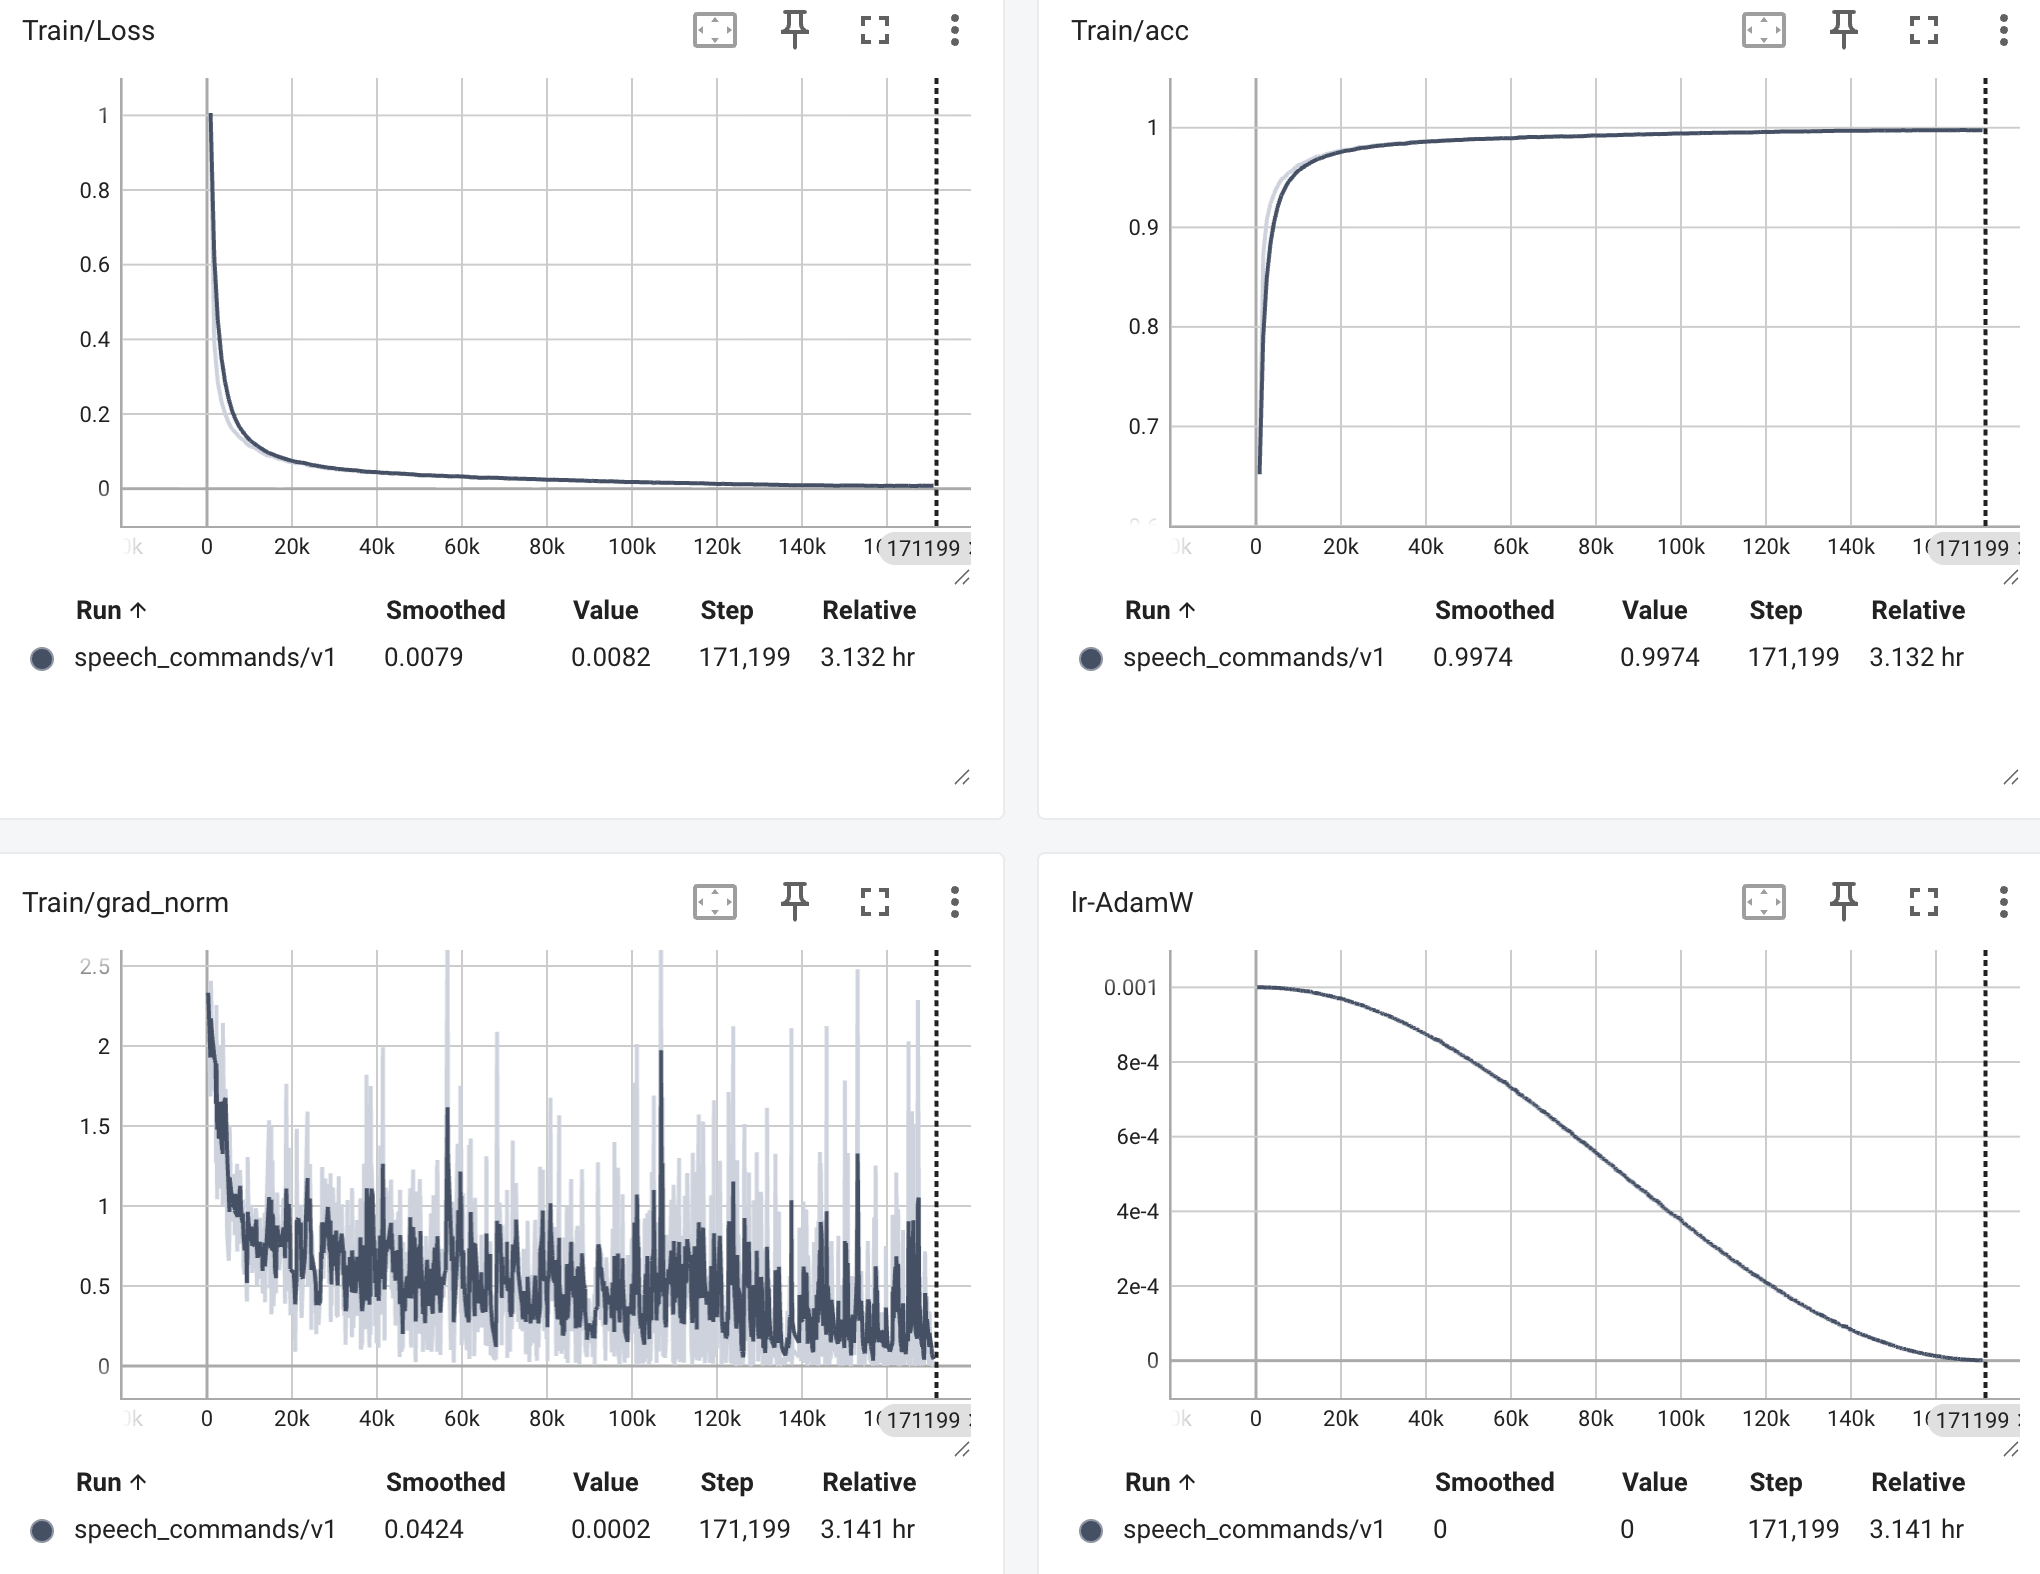
\includegraphics[width=\colfigwidth]{images/train_curves_grad_norm}
  \caption{Training loss, accuracy, learning rate decay, and gradient norm.}
  \label{fig:train}
\end{figure}

\begin{figure}[t]
  \centering
  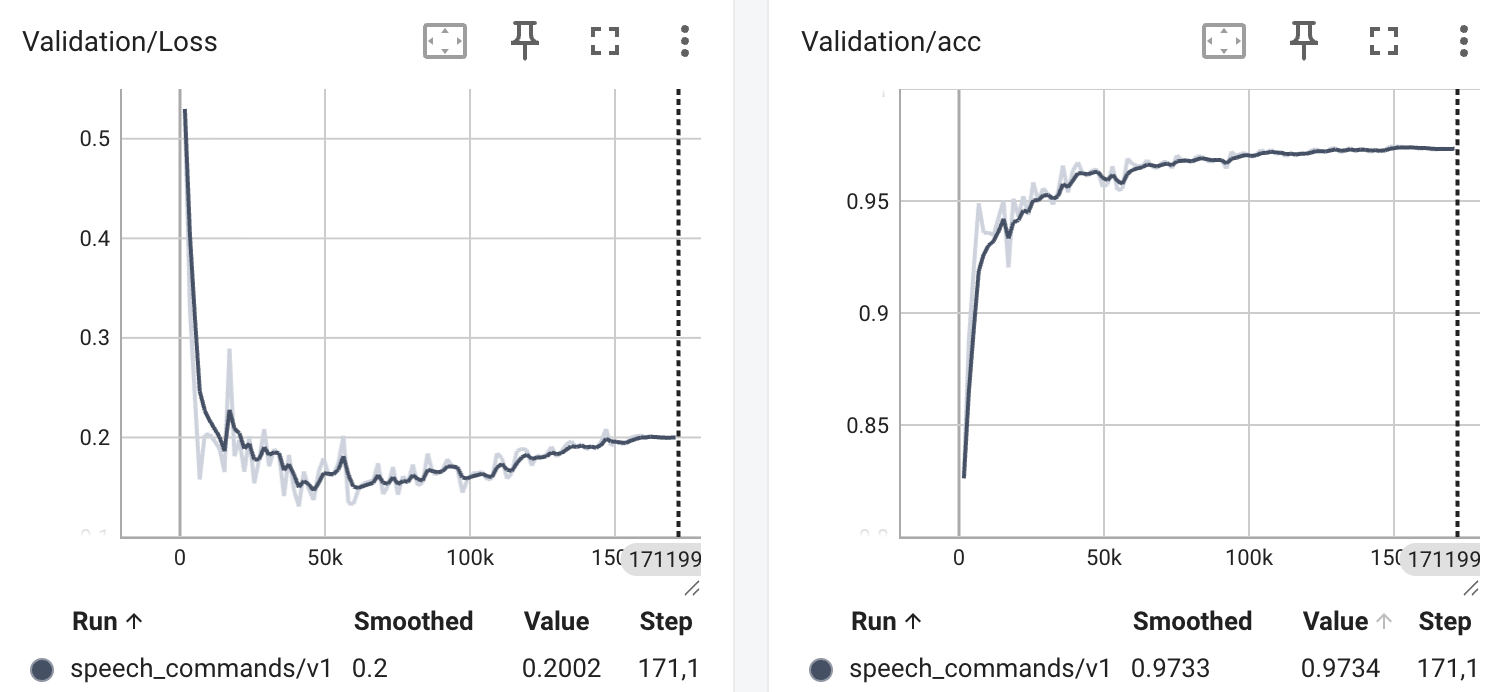
\includegraphics[width=\colfigwidth]{images/valid_curves}
  \caption{Validation loss and accuracy.}
  \label{fig:valid}
\end{figure}

\begin{figure}[t]
  \centering
  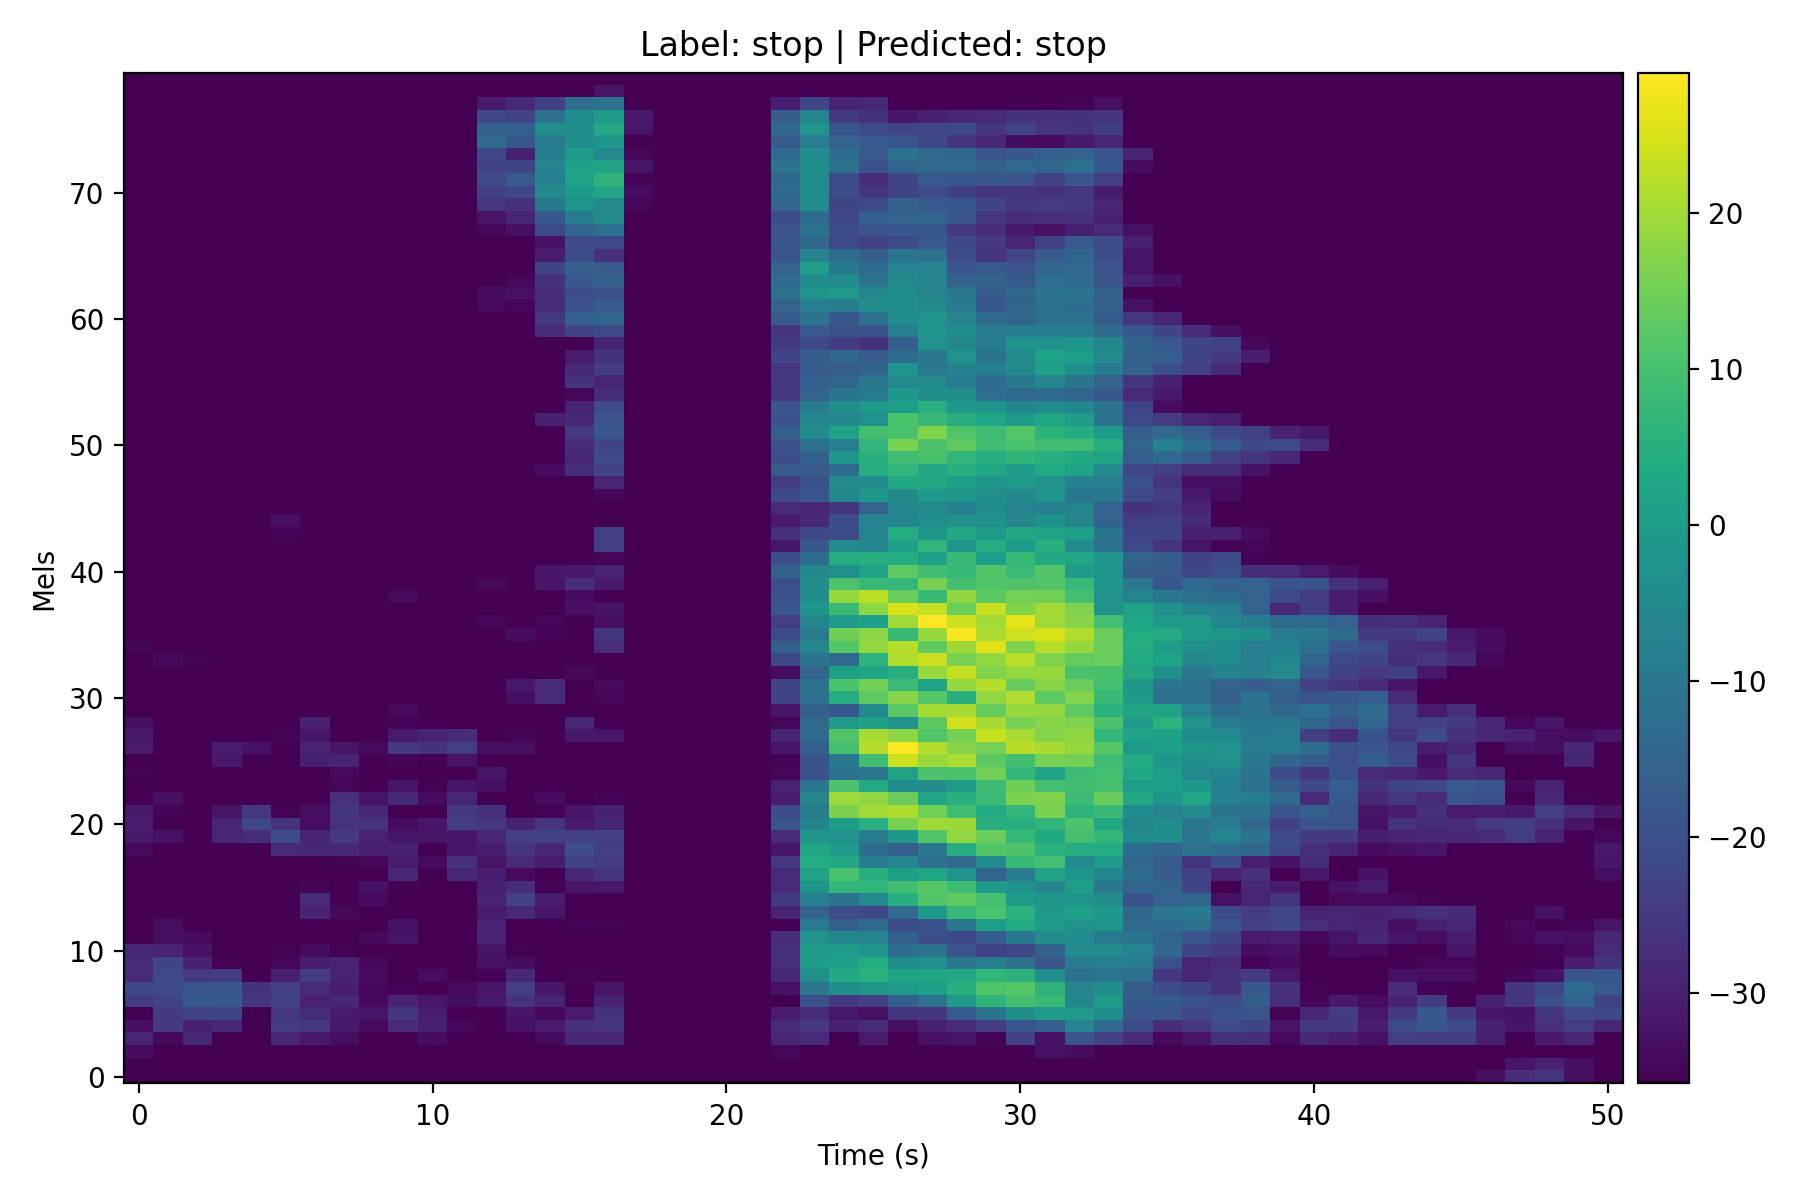
\includegraphics[width=\colfigwidth]{images/train_timemask}
  \caption{Training-time waveform TimeMask augmentation.}
  \label{fig:timemask}
\end{figure}

\begin{figure}[t]
  \centering
  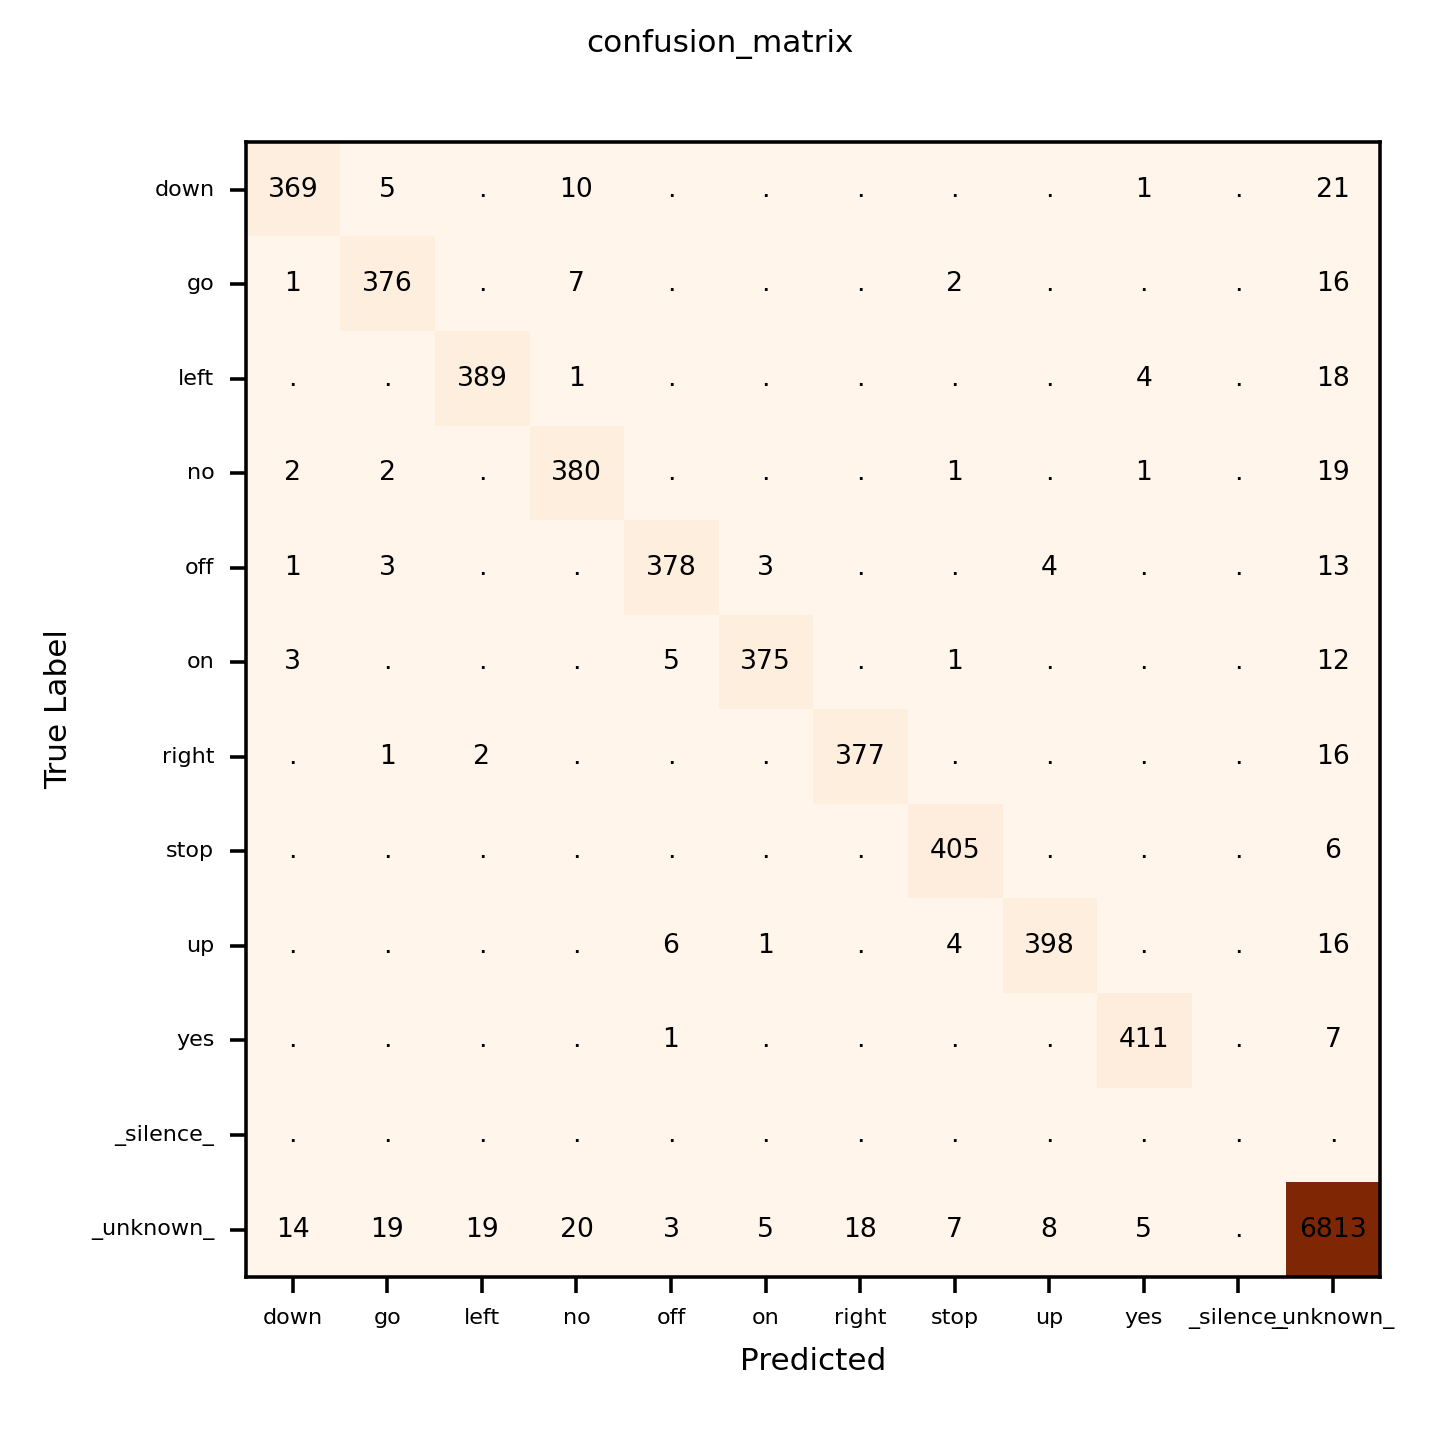
\includegraphics[width=\colfigwidth]{images/confusion_metrix}
  \caption{Confusion matrix on the test set.}
  \label{fig:cm}
\end{figure}

\begin{figure}[t]
  \centering
  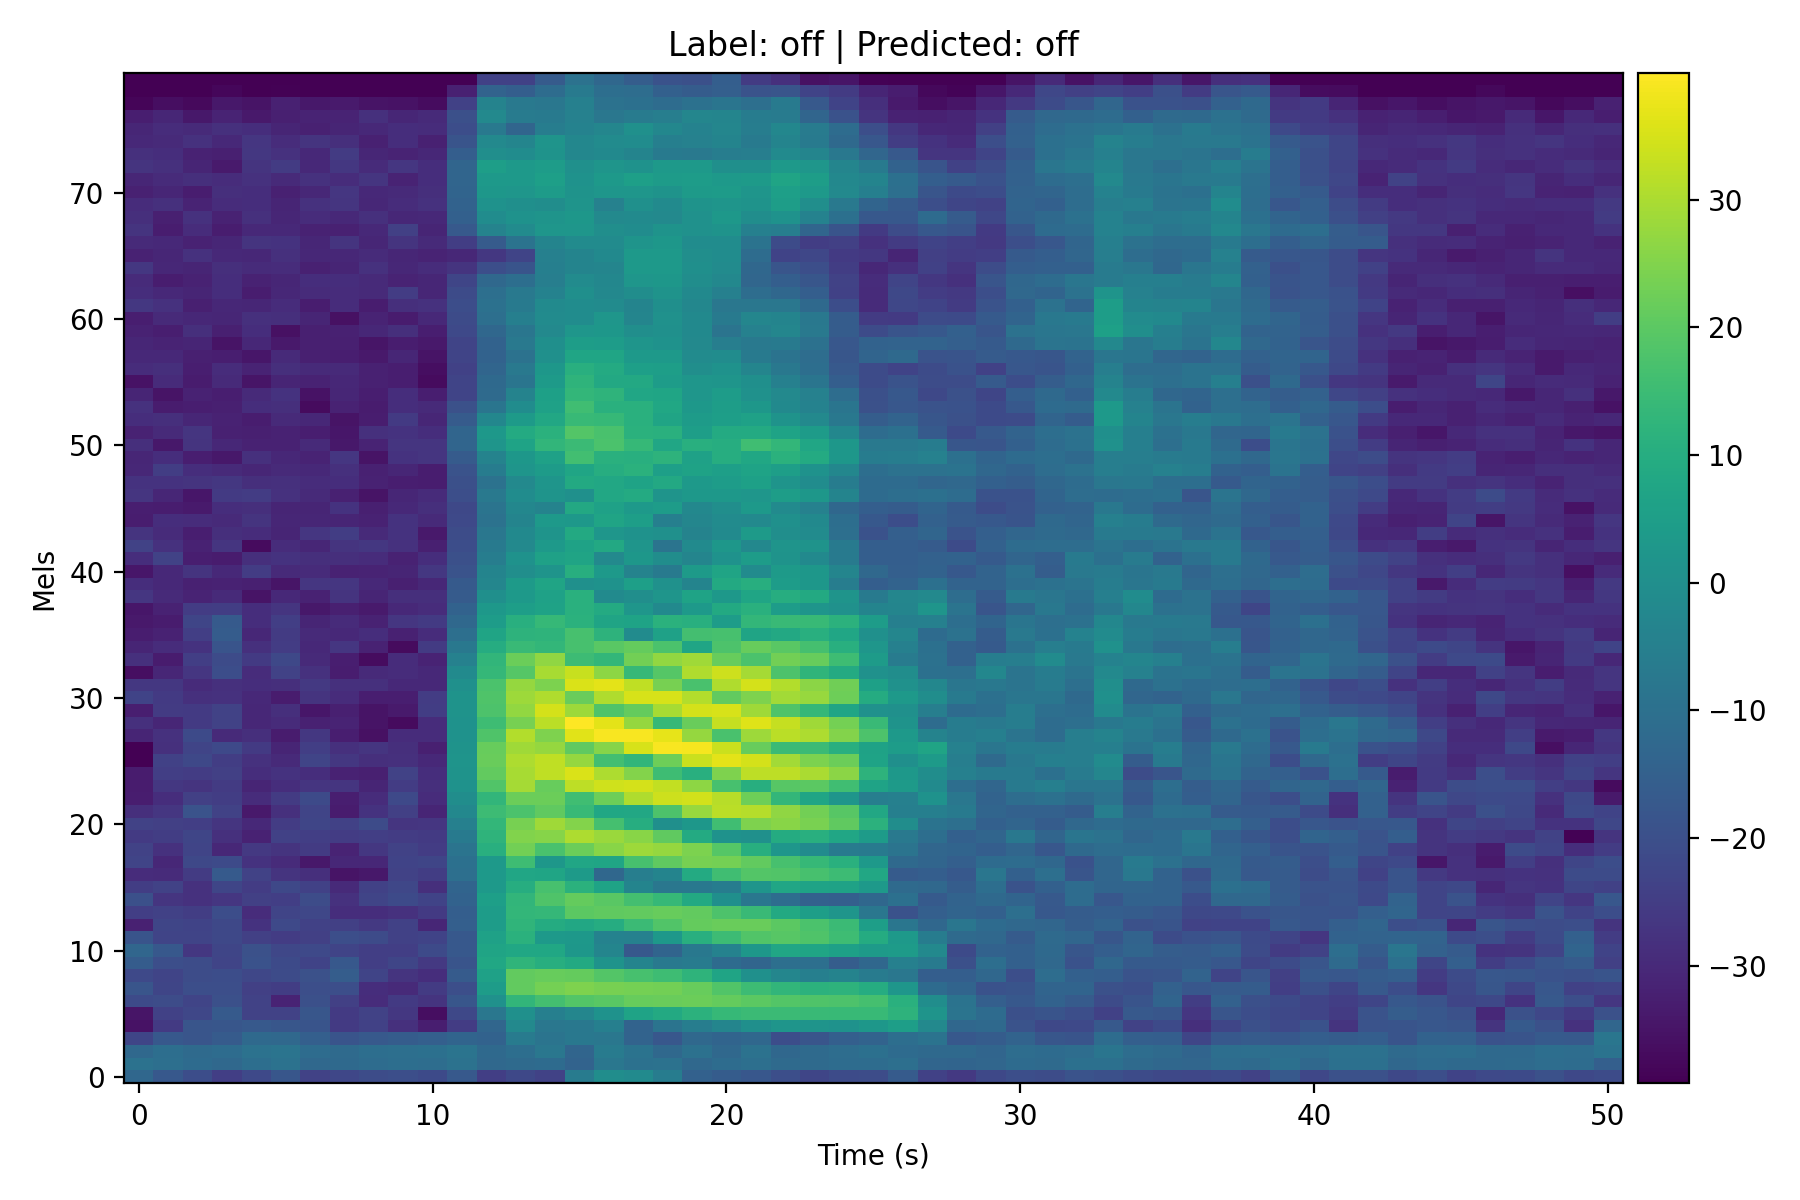
\includegraphics[width=\colfigwidth]{images/test_off}
  \caption{Testset example: correctly predicted label \texttt{off}.}
  \label{fig:test_off}
\end{figure}

\begin{figure}[t]
  \centering
  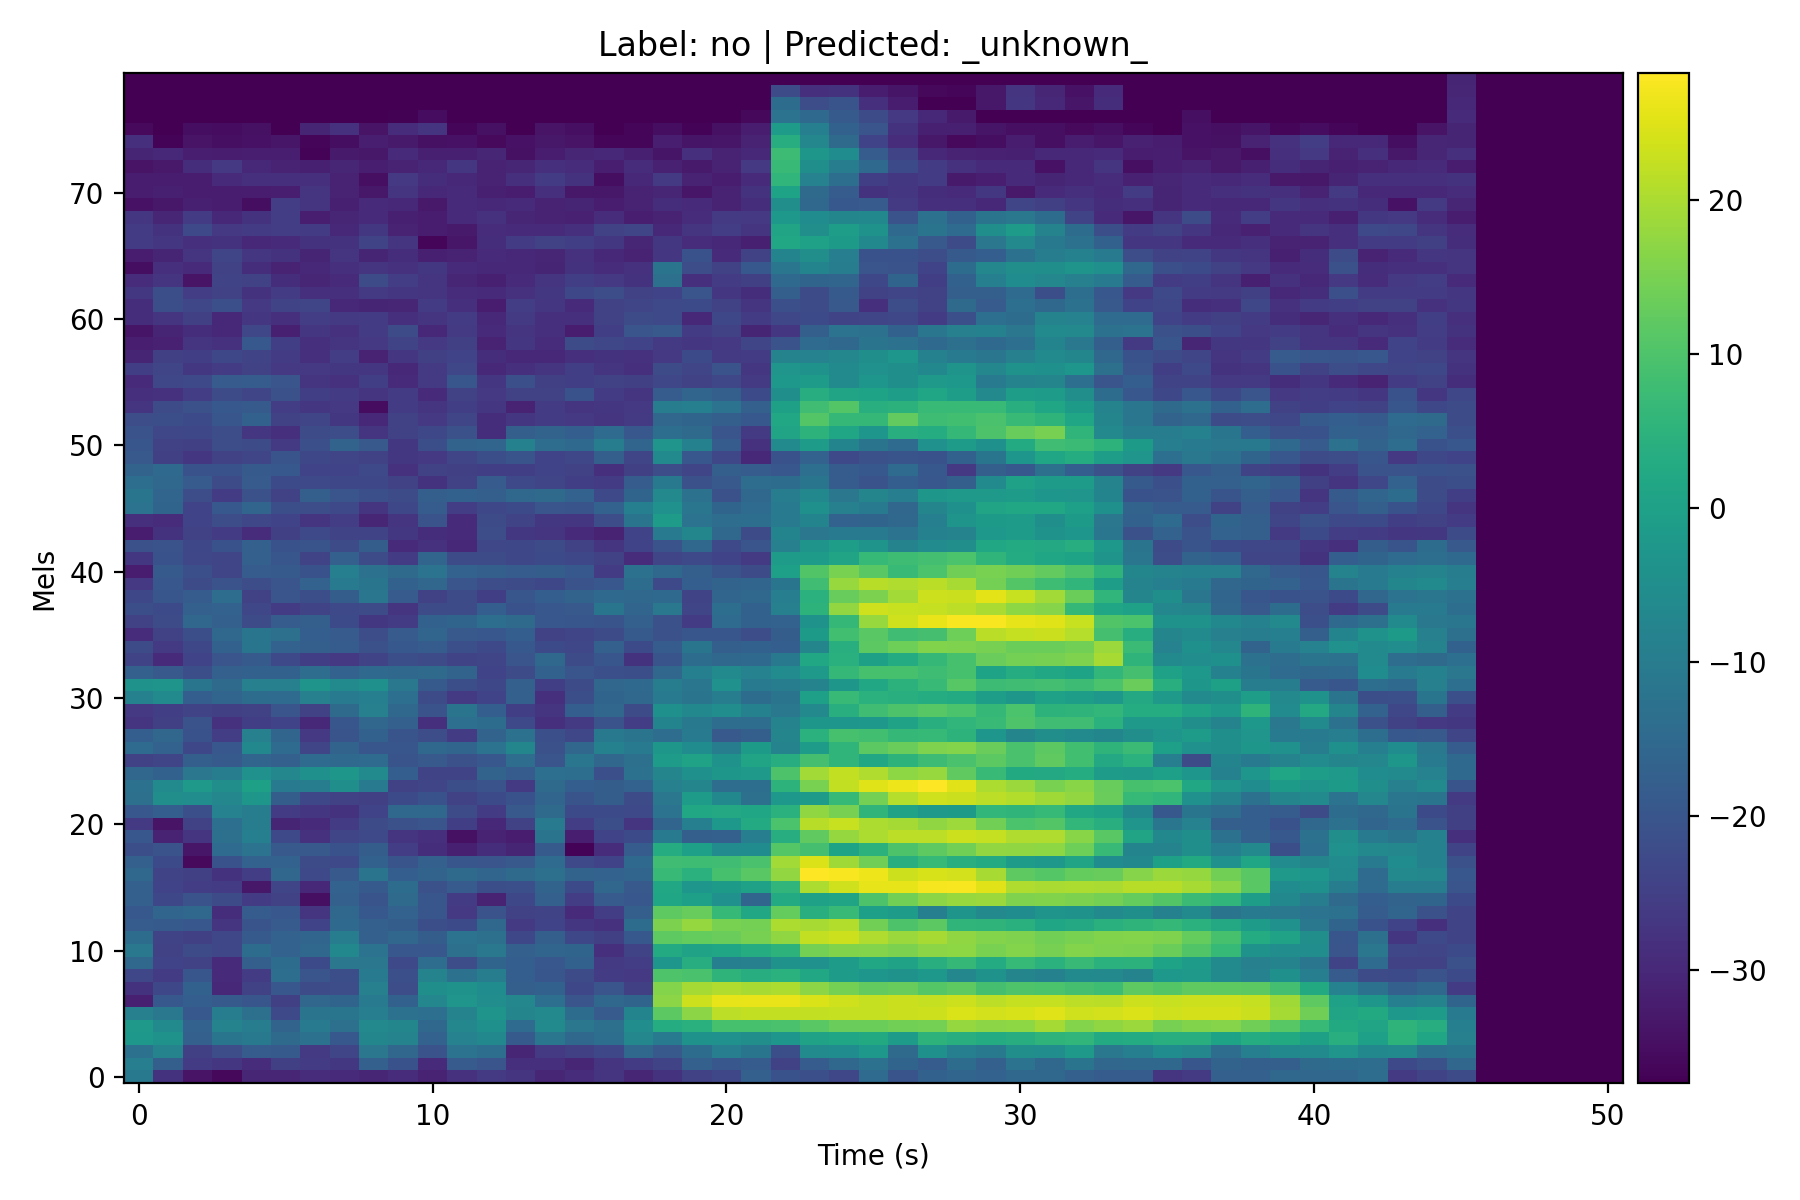
\includegraphics[width=\colfigwidth]{images/test_no_incorrect}
  \caption{Testset example: incorrectly predicted label \texttt{unknown}, target label \texttt{no}.}
  \label{fig:test_no}
\end{figure}

\section{Conclusion}

I was able to achieve the required test accuracy of $0.9697$ with assignment requirements. The confusion matrix shows that the model is able to correctly classify, with little confusion between classes. The major point of confusion is between \texttt{unknown} and \texttt{silence}. With more time, I'd like to explore more data augmentation techniques (pitch and formant purtubation, RIR augmentation, noise augmentation, etc.) and and encoder pretraining on large unlabeled dataset (similar to Wav2Vec2), this would help the model to generalize better to unseen data and improve the accuracy.

\begin{thebibliography}{9}

\bibitem{audioloader}
K.~W. Cheuk, \emph{AudioLoader}: PyTorch speech/music datasets, GitHub repository, \url{https://github.com/KinWaiCheuk/AudioLoader}.

\bibitem{nnaudio_tutorial}
K.~Y. Heung, \emph{nnAudio} KWS tutorial with PyTorch Lightning, GitHub repository, \url{https://github.com/heungky/nnAudio_tutorial}.

\end{thebibliography}

\end{document}